\documentclass[12pt]{article}
\usepackage{amsmath}
\usepackage{graphicx}
\usepackage{hyperref}
\usepackage[latin1]{inputenc}

\title{Progetto di Programmazione}
\author{Nome : n. matricola}
\date{settembre 2023}

\begin{document}
\maketitle

\begin{figure}[h]
    \centering
    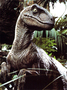
\includegraphics{raptor.jpg}
    % qui ci va il logo dell'unibo ma ora non me lo fa mettere
\end{figure}

\newpage


\section*{Suddivisione dei compiti}
\subsection*{Davide}
\begin{itemize}
    \item Menu principale
    \item Menu di pausa
\end{itemize}
 
\subsection*{Elia}
\begin{itemize}
    \item Personaggio 
    \item Nemici
\end{itemize}

\subsection*{Matteo}
\begin{itemize}
    \item Artefatti
    \item Sistema di combattimento
\end{itemize}

\subsection*{Mattia}
\begin{itemize}
    \item Creazione e gestione delle stanze 
    \item Strutture dati per la loro memorizzazione
    \item Grafica
\end{itemize}

\newpage
\section*{Scelte implementative}
\subsection*{Il Gioco}
La classe Menu gestisce il menù principale, mentre la classe Game si occupa di gestire tutto ciò che riguarda il gioco.
% brutto come è scritto
Game comprende 3 finestre (per la grafica delle stanze, delle staistiche del personaggio e per il punteggio), il personaggio (Hero), l'indice delle stanze e un puntatore alla stanza corrente.

\subsection*{Il Personaggio}
\subsection*{Le Stanze}
\subsection*{I Nemici}
\subsection*{Gli artefatti}
\subsection*{Il sistema di combattimento}

\end{document}












